\chapter{Fluxograma de decisão}
\label{cap:fluxograma}

A \cref{fig:fluxograma} apresenta, de forma simplificada, o fluxo de inferência e tomada de
decisão seguido pelo sistema durante cada ciclo da simulação. O processo inicia-se com a
leitura dos valores provenientes dos sensores, que são posteriormente processados e utilizados
para avaliar as condições presentes na situação atual.

% Figura alta: ocupa uma página própria ([p]), logo a seguir ao texto.
\begin{figure}[p]
  \centering
  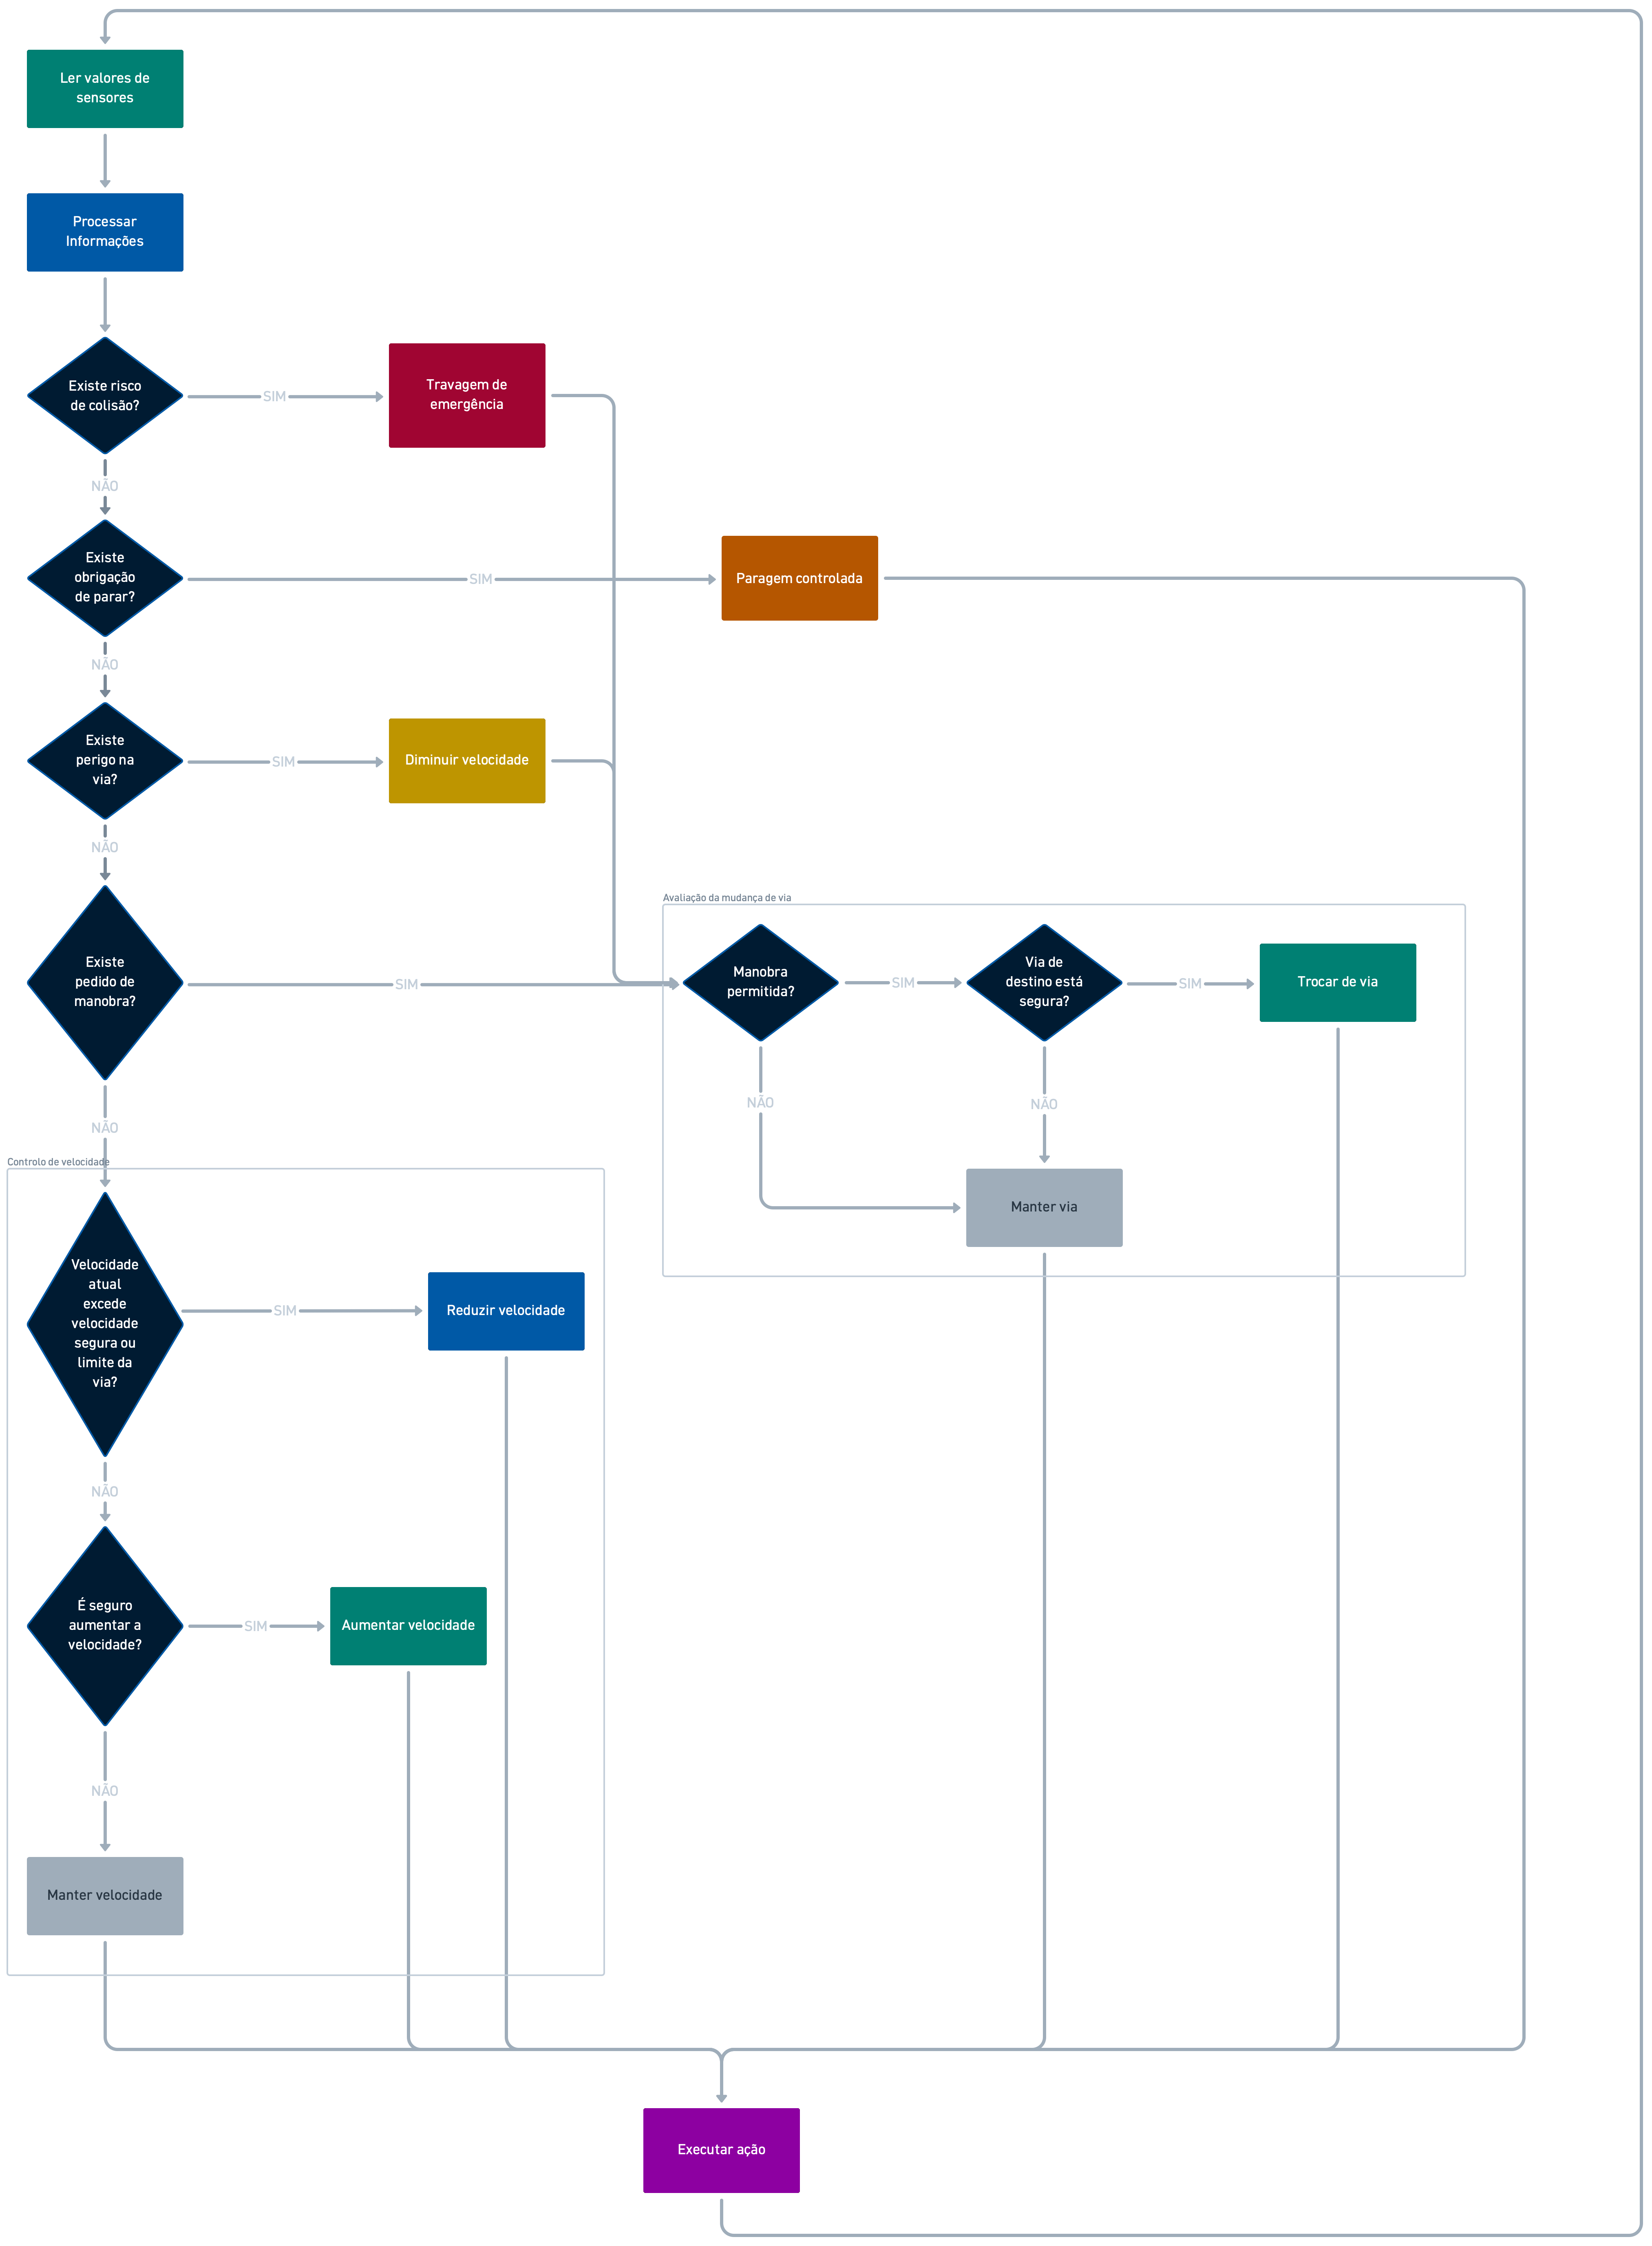
\includegraphics[width=\textwidth,height=0.88\textheight,keepaspectratio]{figuras/fluxograma1.png}
  \caption{Fluxograma de inferência e tomada de decisão em cada ciclo da
    simulação}
  \label{fig:fluxograma}
\end{figure}

A primeira verificação corresponde à existência de risco de choque. Caso seja identificado
esse risco, o sistema propõe uma travagem de emergência. Na ausência dessa condição, é verificada
a existência de uma obrigação de parar, podendo ser proposta uma paragem controlada. Caso também
não exista essa obrigação, o sistema verifica a existência de um perigo na via. Quando é
identificado um perigo, é proposta uma diminuição de velocidade e, em seguida, uma troca de via.

Na ausência de perigo, é verificada a existência de um pedido de manobra. Caso exista, o sistema
inicia a avaliação da mudança de via, verificando primeiro se a manobra é permitida e,
posteriormente, se a via de destino está segura. Quando ambas as condições são satisfeitas, é
proposta a troca de via. Caso a manobra não seja permitida ou a via de destino não seja
considerada segura, o sistema propõe manter a via.

Quando não existe um pedido de manobra, o processo segue para o controlo da velocidade. Nesta
fase, é verificado se a velocidade atual excede a velocidade segura ou o limite da via. Caso
exceda, é proposta uma redução da velocidade. Caso contrário, o sistema avalia se é seguro
aumentar a velocidade. Se essa condição for satisfeita, é proposta uma aceleração, caso contrário,
a velocidade é mantida.

As diferentes decisões propostas convergem posteriormente para a execução da ação selecionada.
A ação executada altera o estado do veículo e, consequentemente, as condições observadas no
ambiente. O ciclo reinicia-se então com uma nova leitura dos sensores, permitindo que o sistema
acompanhe continuamente a evolução da situação e reavalie a decisão em função dos novos dados
disponíveis.

